%%%%%%%%%%%%%%%%%%%% author.tex %%%%%%%%%%%%%%%%%%%%%%%%%%%%%%%%%%%
%
% sample root file for your "contribution" to a contributed volume
%
% Use this file as a template for your own input.
%
%%%%%%%%%%%%%%%% Springer %%%%%%%%%%%%%%%%%%%%%%%%%%%%%%%%%%


% RECOMMENDED %%%%%%%%%%%%%%%%%%%%%%%%%%%%%%%%%%%%%%%%%%%%%%%%%%%
\documentclass[graybox]{svmult}

% choose options for [] as required from the list
% in the Reference Guide

\usepackage{mathptmx}       % selects Times Roman as basic font
\usepackage{helvet}         % selects Helvetica as sans-serif font
\usepackage{courier}        % selects Courier as typewriter font
\usepackage{type1cm}        % activate if the above 3 fonts are
                            % not available on your system
%
\usepackage{makeidx}         % allows index generation
\usepackage{graphicx}        % standard LaTeX graphics tool
                             % when including figure files
\usepackage{multicol}        % used for the two-column index
\usepackage[bottom]{footmisc}% places footnotes at page bottom

%
\usepackage{url}
\usepackage{amssymb}

% see the list of further useful packages
% in the Reference Guide

\makeindex             % used for the subject index
                       % please use the style svind.ist with
                       % your makeindex program

%%%%%%%%%%%%%%%%%%%%%%%%%%%%%%%%%%%%%%%%%%%%%%%%%%%%%%%%%%%%%%%%%%%%%%%%%%%%%%%%%%%%%%%%%

\begin{document}

\title*{Performance Evaluation Experiments of Bitcoin SV Scaling Test Network}
% Use \titlerunning{Short Title} for an abbreviated version of
% your contribution title if the original one is too long
\author{Akihiro Fujihara and Takaaki Yanagihara}
% Use \authorrunning{Short Title} for an abbreviated version of
% your contribution title if the original one is too long
\institute{Akihiro Fujihara \at Chiba Institute of Technology, 2-17-1 Tsudanuma, Narashino, Chiba 275-0016, JAPAN, \email{akihiro.fujihara@p.chibakoudai.jp}
\and Takaaki Yanagihara \at Chiba Institute of Technology, 2-17-1 Tsudanuma, Narashino, Chiba 275-0016, JAPAN, \email{s1522313qq@s.chibakoudai.jp}}
%
% Use the package "url.sty" to avoid
% problems with special characters
% used in your e-mail or web address
%
\maketitle

\abstract{
The Bitcoin SV Scaling Test Network (STN) is an experimental network for solving the scalability problem of Bitcoin with On-chain technology.
A large amount of transactions are always transmitted on P2P networks, and experiments are conducted to generate huge blocks.
In this study, by constructing the STN node, the occupancy rate of transaction processing and the branch probability of the blockchain are estimated. 
As a result, the estimated occupancy rate was about 1.04 and the estimated branch probability was 8.5\%.
In addition, the transaction processing performance was experimentally evaluated by transferring transactions including the OP\_RETURN script at a high frequency of once per minute for a period of one week.
As a result, the probability of the transaction being processed into BC was 98\%.
It was also confirmed that the latency distribution taken for transactions to be processed in tended to follow a power-law distribution at the tail.
From the above, the consideration by the queueing theory with priority seems to be effective even in STN.
}


\section{Introduction}
\label{sec:intro}

ブロックチェーンは1990年代にHaberとStornettaによって発表された電子書類の分散タイムスタンプ・サービスに関する理論研究に起源がある
\cite{HS1991,BHS1993,HS1997}.
当時はインターネットが十分に発達しておらず,提案システムの実環境での利用は困難であった.
2008年にビットコイン\cite{nakamoto}が登場する頃には実環境が整っており,翌2009年1月3日には提案システムの稼働も始まった.
これ以降,ビットコインは稼働し続けている.
このビットコインの実績と共に,分散タイムスタンプ・サービスと本質的に同じ技術がブロックチェーン
(Blockchain, BC)という言葉に変わり,注目を集めるようになった.

ビットコインによって誕生した新アイデアは,BCではなく,Nakamoto Consensusと呼ばれる,ネットワークに参加する不特定多数のノードがBCについて合意形成を行う仕組みにあった.
合意形成によって同じ状態を持ち合う技術は,ビットコインの登場以前から知られていたが,仲基合意は作業証明(Proof of Work, PoW)\cite{DN1993,JJ1999},最長チェーン規則,インセンティブ機構といった複数の仕組みを組み合わせることにより,インターネット規模での不特定多数のノード間で合意形成が可能な仕組みを生み出した点で斬新であった.

Bitcoinの本質的に新しい利用価値は,取引にかかる手数料を極度に安くする事によって実現できる,1円や1セント以下のMicropaymentにある.
このことによってインターネット上の様々なサービスの利用時に,ほぼ0に近い(人々が支払いを行ったことを気にしないレベルの)課金を沢山のユーザから集めることができる.
つまり超少額決済は,これまでにない新しい分散型経済の仕組みを作ることができる潜在能力を持っている.
しかし,現時点でBitcoin Core (BTC) \cite{btc} は電子貨幣システムとして普段の支払いに利用されるわけではなく,投機目的の価値の貯蔵システムと化してしまった.
その背景には,現状のビットコインでは多数の超少額決済の実行が事実上困難であるという理由がある.

BTCのブロックサイズの上限は1MBに決まっている.
これより大きなサイズのブロックは不当なものとみなされ,マイナーに拒否される.
またビットコインの平均ブロック生成時間は10分になるように難易度調整アルゴリズムによって制御されている.
従って,平均10分に1MB以下のブロックに取り込めるだけの取引しか処理することができない.
これは1秒あたり5〜7取引しか処理できない計算になる.
単純に平均ブロック生成時間を10分より短くしたり,ブロックサイズの上限を1MBより大きくすれば,この問題が解決するように思われる.
しかし,ブロックサイズを大きくすると,ブロックをP2Pネットワーク上の全ノードに転送して共有する過程により時間がかかってしまう.
従って,平均ブロック生成時間を10分より長くしないとブロックがP2Pネットワーク全体に行き渡る前に別のブロックが生成される確率が上がる.
従って,単純にブロックサイズを大きくしてもBCの分岐を引き起こすことになる.
分岐が起こるとProof of Work (PoW)を行ってブロックを生成するノードのハッシュレートが二種類のブロックの生成に分断されてしまう.
これは将来的に排除されてしまうブロックの生成に大量のハッシュパワーをかけてしまうことを意味し,ネットワーク全体のブロック生成効率も下がる.
平均ブロック生成時間を10分よりも短くしても,同じくBCの分岐が起こりやすくなり,同様の困難が生じる.
これらの理由により,単位時間あたりの取引処理性能を向上することには技術的な困難がある.
この技術的な課題のことをスケーラビリティ問題と呼ぶ.


ビットコインのスケーラビリティ問題を解決する方法も様々なものが提案されている
\cite{ZHZB2020,Fujihara2018,Fujihara2019,Fujihara2020,YF2021a,YF2021b}.
その中でもLightning network\cite{PD2016}のように,BC外で多量の取引をまとめて実行し,その最終結果のみをBCに書き込むことで,ブロックに取り込む取引量を減らす手法に注目が集まっている.
この手法はBC外の仕組みを駆使してスケーラビリティ問題を回避することから,Off-chainのスケー
リング技術と呼ばれる.
Off-chain技術は一見良いように見えるが,個々の取引処理がBCに残らない.
従って,Off-chainで処理した取引の改ざんが可能になってくる.

またビットコインは,ダークネット・マーケットにおける違法な取引を行う手段として利用されてきた歴史がある.
しかし,近年これらのマーケットの支配人や利用者が逮捕される事例が数多く報告されている
\cite{silkroad,alphabay,welcome2video}.
これらの逮捕はビットコインが全取引を改ざん耐性を持たせて公開している為に,法的な証拠として利用可能であることに起因する.
この観点から考えると,Off-chain技術が普及するほど,政府等が追跡して監査することが不可能な取引が増えてしまい,ダークネット・マーケットにおける違法な取引の取り締まりが難しくなったり,マネー
ロンダリングの温床となりうる.
法と倫理とのバランスを考えた時,究極的にはBC上で全取引を処理するOn-chain技術によってスケーラビリティ問題を解決することが求められる.

On-chainでスケーラビリティ問題を解決する為には,BCが分岐しないようにうまく制御しながら平均ブロック生成時間を短くするか,ブロックサイズを大きくする必要がある.
bloXroute\cite{bloX}は,Blockchain Distribution Network (BDN)という名称の,より大きなブロックをより短時間で伝搬させることが可能なネットワーク層をP2Pネットワークに接続することで,ブロック伝搬速度を改善しようとする提案である.

ブロックサイズを拡大する取り組みはBitcoin SV (BSV) \cite{bsv} Scaling Test Network (STN)で実験的な取り組みが行われている\cite{bitcoinscaling}.
上述の通り,BTCのブロックサイズの上限は1MBであるのに対し,BSVではブロックサイズの上限を撤廃した.
これにより2021年2月9日時点で,24時間あたりの平均取引処理数が1,059 Transactions Per Second (TPS),これまでに採掘された中で最も大きなブロックサイズは2.9GBと報告されている.

本研究ではSTNのノードを構築することで,ブロックサイズの上限を撤廃した環境における取引処理に関するデータ分析や性能評価実験を行った結果について報告する.
本研究の貢献を以下に示す.
%
\begin{itemize}
  \item 待ち行列理論を用いることで取引処理の稼働率の時間変化を調べた.
	その結果,推定稼働率は殆どの時間帯で1を超えていることが分かった.
  \item bitcoin-cliの機能を用いることで,BCの分岐確率の推定を行った.
	その結果,BTCでは分岐確率が約2\%であることが計算されているが,BSV STNでは約8.5\%に増加していることが分かった.
	このことから,P2Pネットワークのノード全体にブロックを転送する時間は約53秒となることも計算により推定できた.
  \item OP\_RETURNスクリプトを含む取引を1分に1回の高頻度で転送した時にBCに取り込まれるまでにかかる時間を実測した.
	その結果,取引がBCに取り込まれる確率は98\%であり,その時間分布は冪分布に従うような傾向が確認できた.
	また優先権付き待ち行列の理論と矛盾しない3/2の冪指数に従う傾向も確認できた.
\end{itemize}
%




\section{Related Works}
\label{sec:rworks}

\subsection{BCの分岐確率の計算}
\label{sec:fork}

ビットコインのブロック生成時間は指数分布に従うことが知られている.
%
\begin{equation}
	F(t) = P(T \le t) = \int_{0}^{t} \lambda e^{-\lambda t'} dt' = 1 - e^{-\lambda t}. \label{eq:exp}
\end{equation}
%
ここでパラメータ$\lambda$は平均ブロック生成時間の逆数である.
ビットコインの場合,平均ブロック生成時間は$1/\lambda=10$分$=600$秒と決まっている.

またBTCのP2Pネットワークの90\%のノードにブロックが拡散されるまでにかかる時間は,Compact Block Relayを適用する以前の場合で$t = \tau_{fork} \fallingdotseq 12$ 秒であることが実測されている\cite{bloX}.
あるブロックがネットワーク全体に拡散される前に,別のブロックが生成された時にBCが分岐してしまう.
従って,ビットコインのBCが分岐する確率は以下のように計算できる.
%
\begin{equation}
  F(\tau_{fork}) = P(T \le \tau_{fork}) = 1 - e^{-\lambda \tau_{fork}} \fallingdotseq \lambda \tau_{fork} = 12/600 = 0.02. 
\end{equation}
%
以上より,BTCのBCの分岐確率は約2\%であることが導かれる.



\subsection{優先権付き待ち行列の理論}
\label{sec:priorityqueue}

優先権の高い客に対して先にサービスを行う優先権付き待ち行列において,稼働率$0 < \rho \le 1$の時,優先権の低い客の待ち時間が冪指数$3/2$の冪分布に従い,その裾野が指数分布のカットオフを持つことが理論解析の結果から知られている
\cite{OB2005}.
%
\begin{eqnarray}
  P(\tau) &=& \frac{A}{\tau^{3/2}} \exp(-\tau/\tau_0), \\
  \tau_0  &=& \frac{1}{\mu (1-\sqrt{\rho})^2}, \\
  \rho    &=& \lambda / \mu.
\end{eqnarray}
%
ただし,$A$は確率分布の規格化定数,$\lambda$は客の平均到着率,$\mu$は平均サービス率である.

また稼働率が超臨界状態$\rho > 1$をとる時も同じ冪分布に従うことが報告されている.
$0 < \rho \le 1$の場合と異なる点は,$1-1/\rho$の割合で待ち時間が無限,つまりサービスを永遠に受けることができない客が現れる.

ビットコインにおける取引がBCに取り込まれるまでにかかる時間は取引手数料に依存した優先権付き待ち行列理論で説明できることが先行研究によって分かっている\cite{KK2019}.
このことから,BSV STNにおいても取引がBCに取り込まれるまでにかかる時間分布も同様の性質を持つことが期待される.




\section{Bitcoin Scaling Test Network}
\label{sec:stn}

ビットコインのスケーラビリティ問題をOn-chain技術で解決する為の実験場として,BSVはRegTest, Testnet以外の第3のテストネットとしてSTNを立ち上げた.
Testnetでは取引数が少ない為,ブロックサイズは小さい傾向にあるが,STNでは巨大ブロックを作るために大量の取引が定期的に送信されている.
STNの未確認(=BCに取り込まれていない)取引件数の時間変化を図\ref{fig:unconfirmed_tx}に示す.
%
\begin{figure}[t]
  \vspace{-45mm}
  \begin{center}
    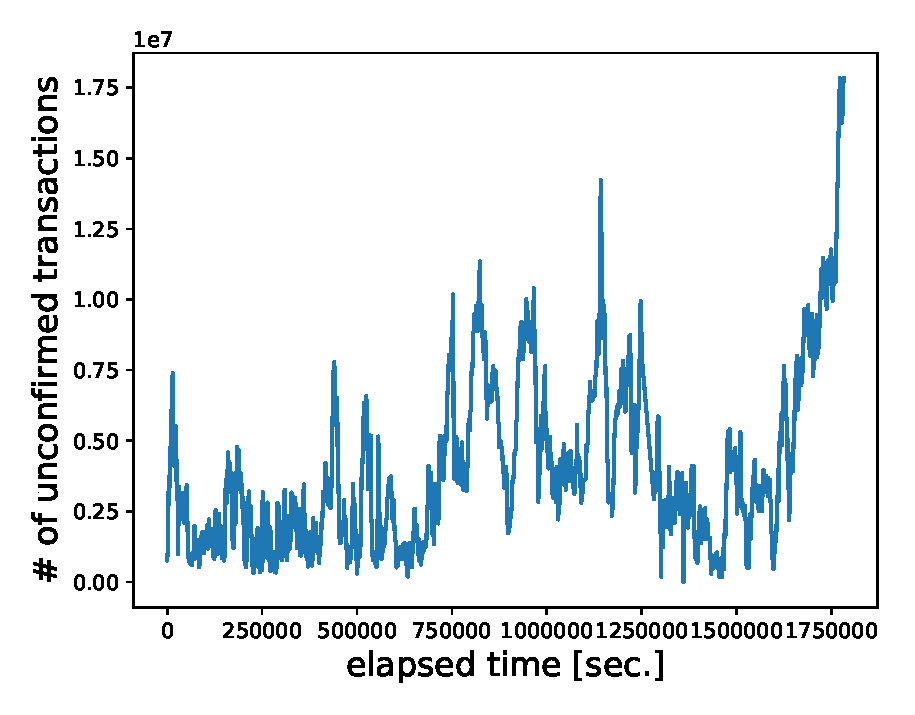
\includegraphics[width=85mm]{time_vs_tx-plot.eps}
  \end{center}
  \vspace{45mm}
  \caption{STNの未確認取引件数の時間変化}
  \label{fig:unconfirmed_tx}
  %  \ecaption{english caption is here}
\end{figure}
%


この図を作成する元となったデータはwhatsonchain\cite{woc}で報告されているものを収集して利用している.
図\ref{fig:unconfirmed_tx}より,定常的に1,000,000以上の取引がTransaction poolに存在していることが分かる.
また時々,取引数が10,000,000以上に達することも分かる.
BSVではOP\_RETURNスクリプトの利用をサポートしているが,取引内容の大半は単純にアドレス間の送金になっている.

STNのネットワークは一般に公開されており,誰でもノードを構築してP2Pネットワークに参加することができる.
ただしノード構築の為のシステム要求として,CPUは8〜16コア,メモリは64GB(+64GB Swap),ハードディスクは3TB以上,インターネット接続は上り下りとも1Gbit以上の性能が要求されている.
BCの総容量は2021年2月9日時点で2.4TBとなっている.
BSVのTestnetでは22GB,Mainnetでも284GB程度である為,比較するとBCの容量が非常に大きいことが分かる.
またSTNのBCのブロック高は2021年2月9日時点で15,216となっており,小さい.これは過去にBCの再編成(=ブロック高を下げて再開)を何度か実施している為である.
BSVのgithubの情報では2020年4月と11月にBCの再編成が行われたことが記録されている.

またシステム要求からも分かるが,STNはCPUによるブロック採掘が可能になっている.ブロック採掘の難易度の時間変化を図\ref{fig:difficulty}に示す.
%
\begin{figure}[t]
  \vspace{-45mm}
  \begin{center}
    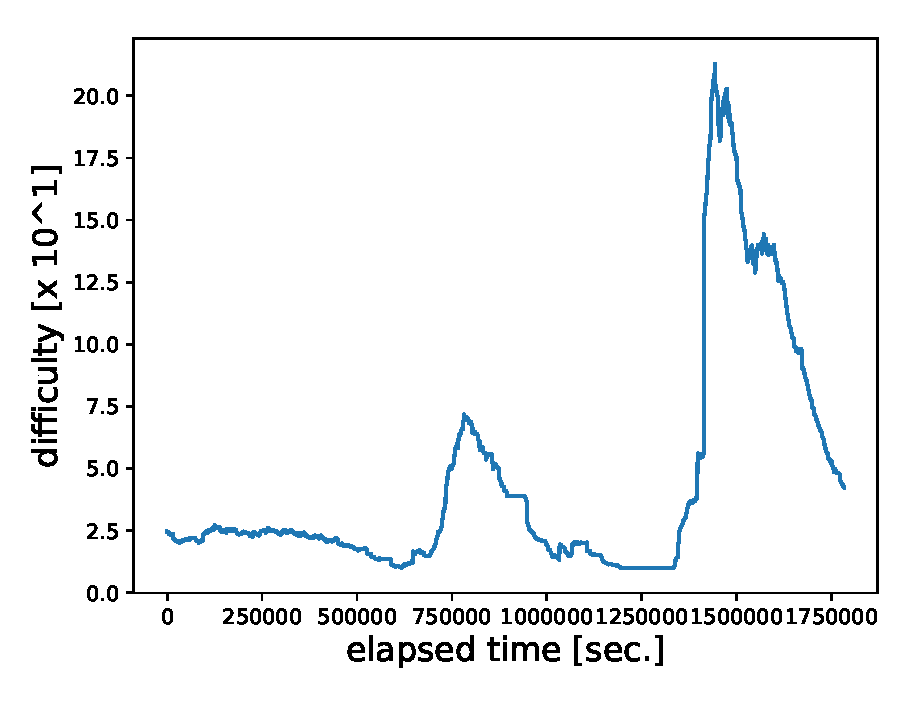
\includegraphics[width=85mm]{time_vs_difficulty-plot.eps}
  \end{center}
  \vspace{45mm}
  \caption{ブロック採掘の難易度の時間変化}
  \label{fig:difficulty}
  %  \ecaption{english caption is here}
\end{figure}
%
難易度は1〜数十の範囲で変化しており,容易に採掘が可能となっている.

STNでは最大ブロックサイズが10GBになるように設定することが推奨されている.
またBitcoin scriptが使用可能なメモリの上限も2GBに設定することが推奨されている.
これまでに採掘されたブロックのサイズ分布を調べた結果を図\ref{fig:block_size}に示す.
%
\begin{figure}[t]
  \vspace{-45mm}
  \begin{center}
    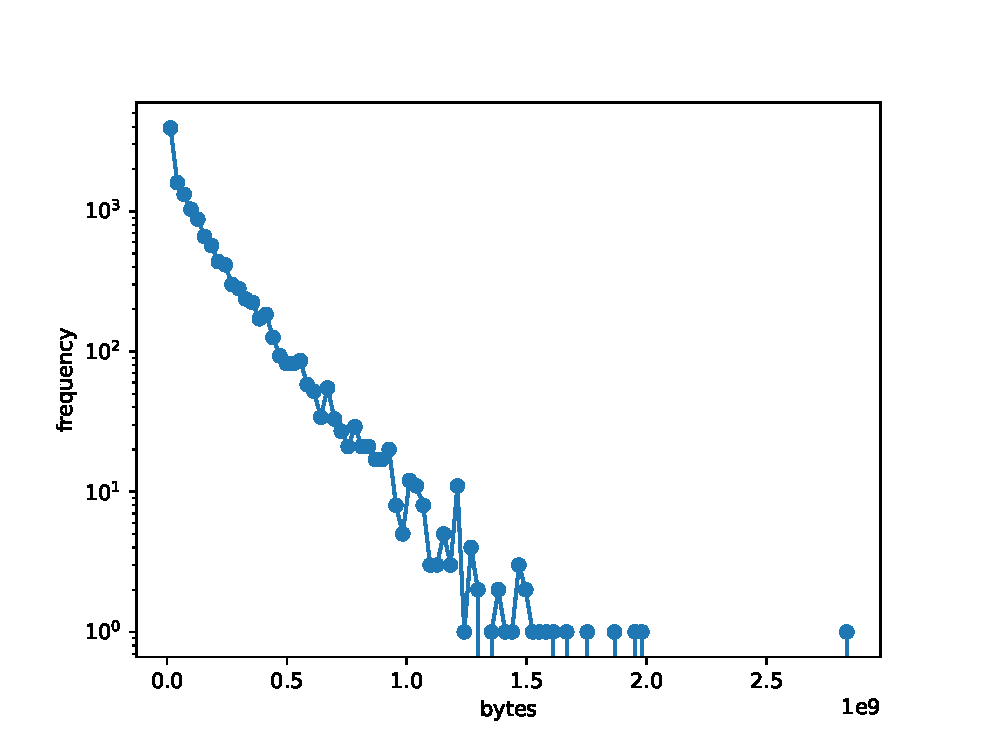
\includegraphics[width=85mm]{bsv_stn-block_bytes-semilogy2.eps}
    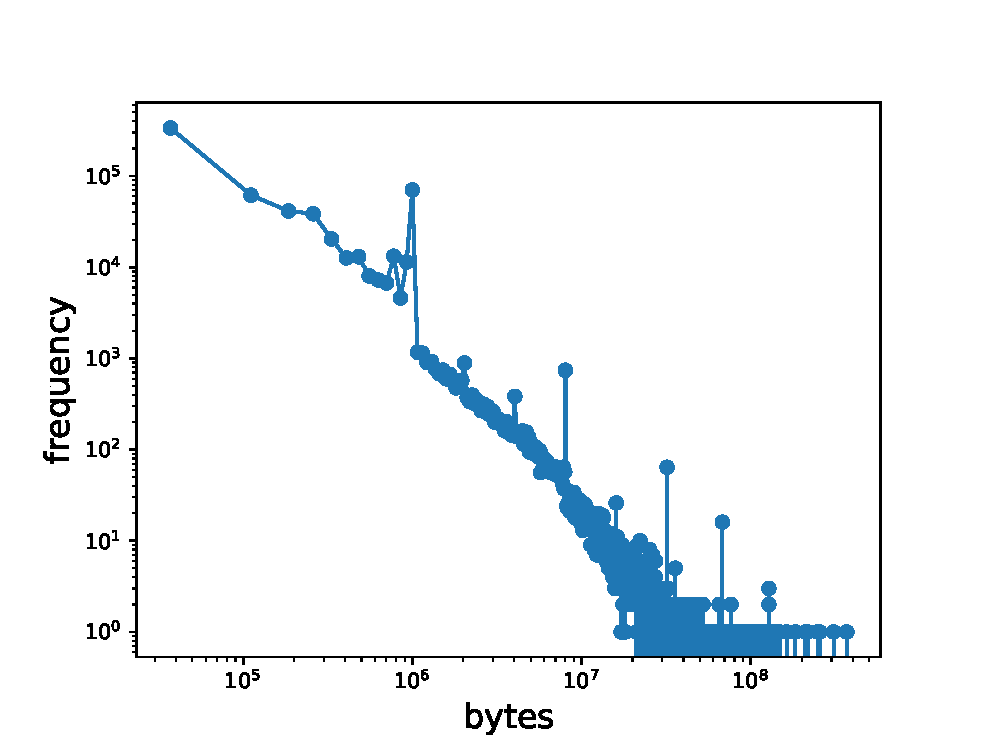
\includegraphics[width=85mm]{bsv_mainnet-block_bytes-loglog.eps}
  \end{center}
  \vspace{45mm}
  \caption{Bitcoin SVにおけるブロックサイズ分布(上図はSTN,下図はMainnet)}
  \label{fig:block_size}
  %  \ecaption{english caption is here}
\end{figure}
%
STNのブロックサイズ分布は指数分布に従っているように見える.
またこれまでに採掘された最大ブロックサイズは2.9GBになっている.
一方,図\ref{fig:block_size}の下図はMainnetでのブロックサイズ分布になるが,興味深いことに指数分布よりも冪分布に従っているように見える.
また冪指数の傾向からPareto-Zipf則(=冪指数2の冪分布)に従っているようにも見える.
STNのコインには市場価値はないが,Mainnetでは市場価値を持つ.
分布にこのような差が生まれる理由については,よく分かっていないが,市場価値を持つコインが入手できる場合,何らかの経済原理が働くことが影響していると考えられる.

BSVは採掘者の評判を評価する観点から採掘したブロックに採掘者IDを記録することを推奨している.
この採掘者IDを参考にしてブロック採掘頻度のランキングを計算した結果を図\ref{fig:minerrank}に示す.
%
\begin{figure}[t]
  \vspace{-45mm}
  \begin{center}
    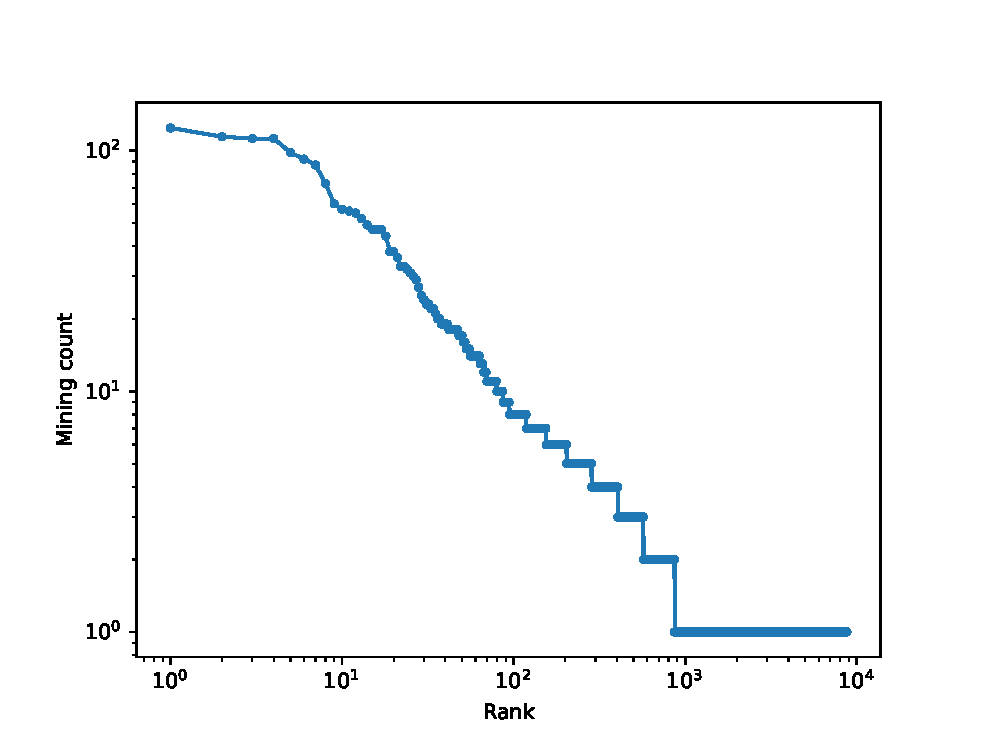
\includegraphics[width=85mm]{bsv_stn-block_miners-ranking-loglog.eps}
  \end{center}
  \vspace{45mm}
  \caption{採掘者IDを参考にして計算したブロック採掘頻度ランキング(STN)}
  \label{fig:minerrank}
  %  \ecaption{english caption is here}
\end{figure}
%
%
\begin{figure}[t]
  %\vspace{-45mm}
  \begin{center}
    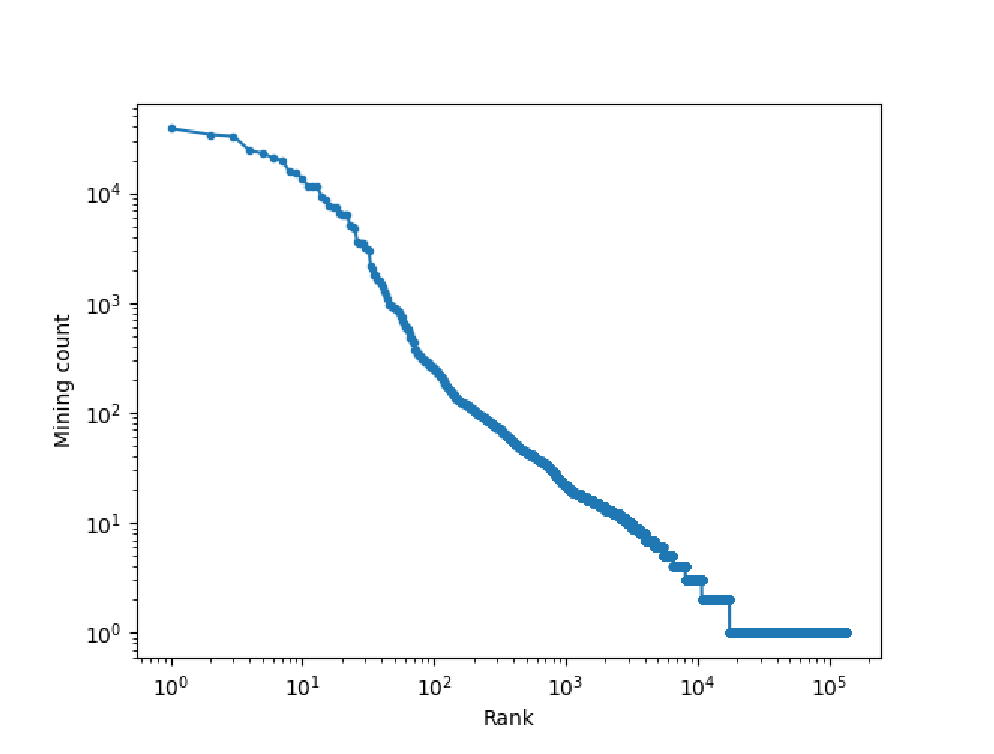
\includegraphics[width=85mm]{bsv_mainnet-block_miners-ranking-loglog.eps}
  \end{center}
  %\vspace{45mm}
  \caption{採掘者IDを参考にして計算したブロック採掘頻度ランキング(Mainnet)}
  \label{fig:minerrank}
  %  \ecaption{english caption is here}
\end{figure}
%
こちらはSTNとMainnetの両方とも冪分布に従っていることが確認できる.



\section{Performance Evaluation Experiments}
\label{sec:experiments}

\subsection{Experiment 1: STNの稼働率}
\label{sec:occupancyrate}

図\ref{fig:unconfirmed_tx}における未確認取引件数の時間変化から,STNの稼働率を推定した.
待ち行列理論に基づいて,STNの推定稼働率$\tilde{\rho}$の時間変化を計算した結果を図\ref{fig:occupancyrate}に示す.
%
\begin{figure}[tb]
  \vspace{-45mm}
  \begin{center}
    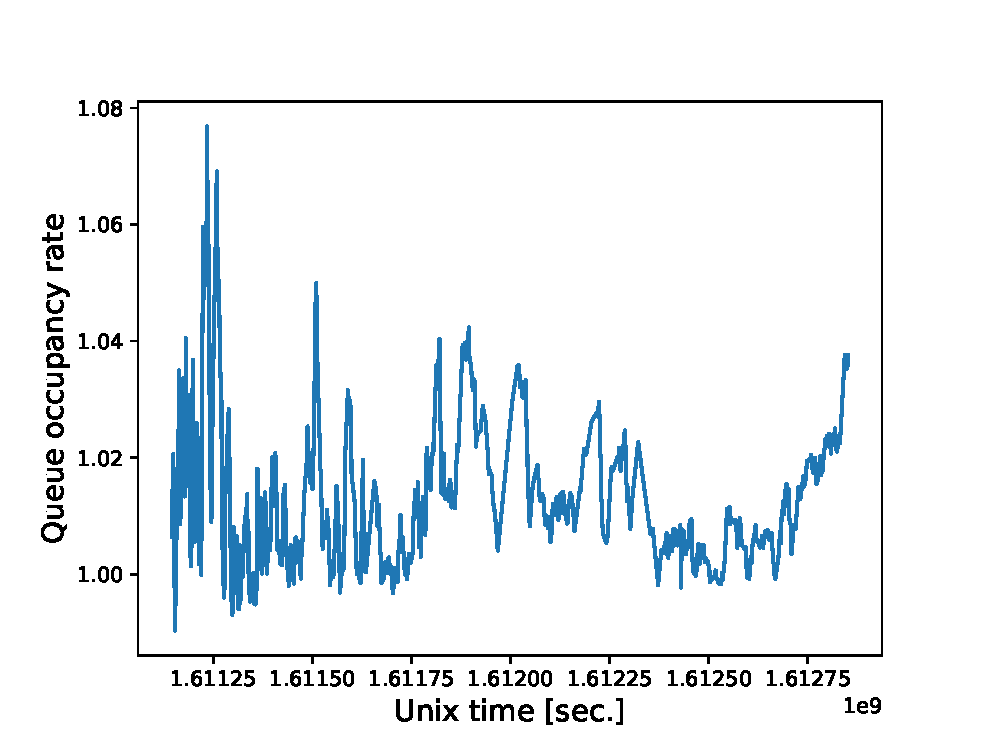
\includegraphics[width=85mm]{bsv_stn-rho-queue_occupancy_rate.eps}
  \end{center}
  \vspace{45mm}
  \caption{STNの推定稼働率$\tilde{\rho}$の時間変化}
  \label{fig:occupancyrate}
  %  \ecaption{english caption is here}
\end{figure}
%
推定稼働率は殆どの時間帯で1を超えていることが分かる.
この結果はBCに取り込まれない取引が存在することを示唆している.
また2020年11月4日〜2021年2月9日までのデータを用いて推定稼働率の時間平均を取ると$\tilde{\rho} \fallingdotseq 1.04$となった.
この結果より,$1-1/\tilde{\rho} \fallingdotseq 0.0387$の確率でBCに取り込まれない取引が出現していると考えられる.



\subsection{Experiment 2: BCの分岐確率の推定}
\label{sec:sork}

STNのノードを構築してP2Pネットワークに接続すると分かるが,大きなブロックが生成されたと思われるタイミングでBCの大きな分岐が起きてSafe modeとなり,bitcoin-cliコマンドを使って送金ができなくなることがある.
また一度大きな分岐が起こると解消までに半日近くかかる場合もある.
そこでbitcoin-cli getinfoのerrorsの値を取得することで分岐が起きている時間から分岐確率を推定する実験を行った.

2020年11月4日〜2021年1月13日の期間において,10秒に1回の頻度でerrorsの値を収集した(合計594,880回).
またBCが分岐している警告が出た回数を数えた.
その結果,以下の2種類の警告が出た.
%
\begin{itemize}
  \item Warning: The network does not appear to fully agree! We received
        headers of a large fork. Still waiting for block data for more details.
	(出現頻度は32,724回, 全体に占める割合は約5.5\%)

  \item Warning: The network does not appear to fully agree! Some miners
        appear to be experiencing issues. A large valid fork has been detected. 
	(出現頻度は17,782回,全体に占める割合は約3\%)
\end{itemize}
%
以上の結果より,分岐確率は約$(5.5+3=)8.5$\%と推定することができる.
これはBTCの約2\%の4倍超であることが分かる.
ちなみに同じ手法でBSV Mainnetの分岐確率を評価すると0\%となった.
また,式(\ref{eq:exp})において$F(t)=0.085$と$\lambda=1/600$を代入した時,$t=\tau_{fork} \fallingdotseq 53$秒となることから,STNにおける平均ブロック転送時間は約53秒になっていると推定することができる.



\subsection{Experiment 3: 取引処理性能の評価実験}
\label{sec:method}

常に沢山の取引がTransaction poolにある状況で,取引がBCに取り込まれるまでにどの程度の時間がかかるかを実験により性能評価した.
実験期間を2021年1月7〜14日の1週間に設定し,期間中に分岐による取引送信ができない場合を除いて常に1分に1回の頻度で,前の1分間にFlightradar24 \cite{flightradar24} のADS-Bデータの収集ノードから千葉工業大学のある津田沼周辺を飛行する民間航空機の位置情報を収集し,OP\_RETURNスクリプト
としてデータを含めた取引の送信を行った.
1取引あたりのサイズは63KB未満になるようにした.
また取引手数料は0.001BSVに固定した.
ちなみにBSVの取引手数料は1 satoshi/byte以上となっている.
昼間は民間航空機が多く飛行する為,取引データのサイズが大きくなるが,夜間は殆ど飛行がない為,書き込むデータが無かった場合は取引の送信は行わなかった.
実験結果に関するその他の詳細情報はGithub に掲載した
\footnote{\url{https://github.com/cit-fujihalab/stn_experiments}}.

実験期間の経過時間と取引が取り込まれたブロック番号の対応関係を図\ref{fig:exp3-1}に示す.
%
\begin{figure}[tb]
  %\vspace{-45mm}
  \begin{center}
    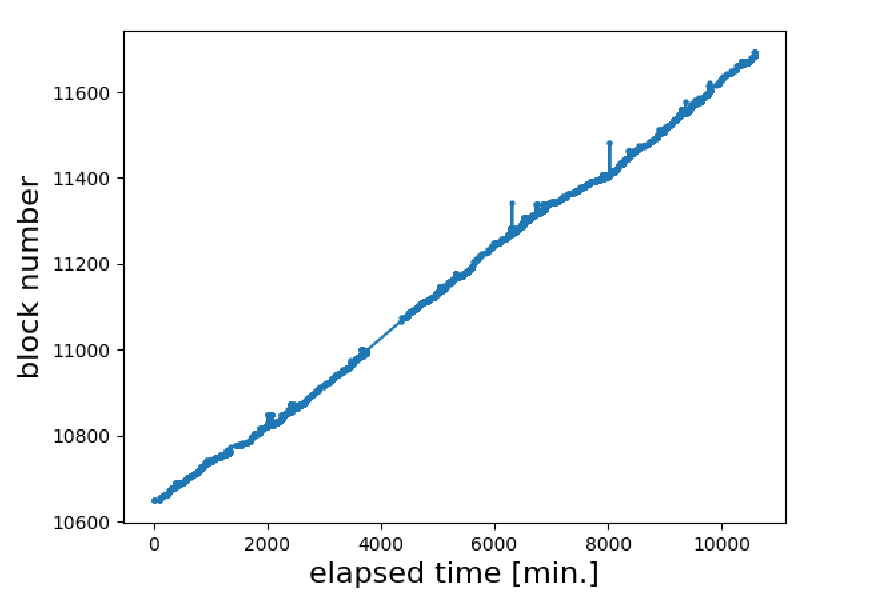
\includegraphics[width=85mm]{exp3-1.eps}
  \end{center}
  %\vspace{45mm}
  \caption{経過時間と取引が取り込まれたブロック番号の対応関係}
  \label{fig:exp3-1}
  %  \ecaption{english caption is here}
\end{figure}
%
経過時間と共に取引が定期的にブロックに取り込まれていることが確認できる.
一方,たまになかなかBCに取り込まれない取引があることも確認できる.

実験期間中に合計6,828取引を送信したが,そのうち104取引はBCに取り込まれなかった.
このことより,取引がBCに取り込まれない確率が$(104/6828 \fallingdotseq) 0.02$と計算できる.
この結果は\ref{sec:occupancyrate}節で計算した$1-1/\tilde{\rho} \fallingdotseq 0.0387$の確率でBCに取り込まれない取引が出現していると推定した結果とほぼ同じ値になっていることが確認できる.

次に取引送信からBCに取り込まれるまでにかかる時間のヒストグラムを図\ref{fig:exp3-2}に示す.
%
\begin{figure}[t]
  %\vspace{-45mm}
  \begin{center}
    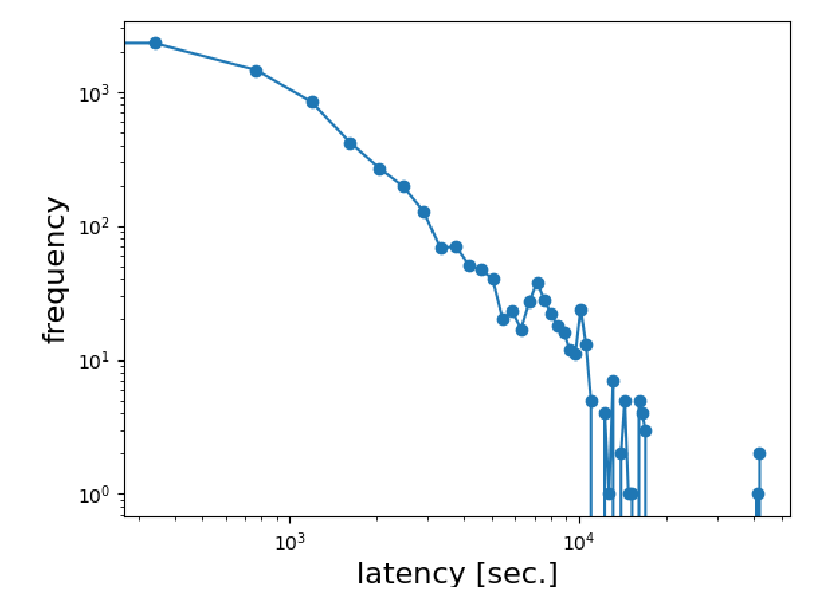
\includegraphics[width=85mm]{exp3-2.eps}
  \end{center}
  %\vspace{45mm}
  \caption{取引送信からBCに取り込まれるまでにかかる時間のヒストグラム}
  \label{fig:exp3-2}
  %  \ecaption{english caption is here}
\end{figure}
%
ブロック生成時間分布が指数分布に従うことから,半日程度の短期間ではBCに取り込まれる時間は指数分布に従うが,1週間程度の長期間になると指数分布から外れてくる.
実際に図\ref{fig:exp3-2}のとおり両対数プロットで直線的な傾向が現れる為,冪分布に従う傾向が現れていることが確認できる.
また冪指数を両対数プロットの傾きから見積もると3/2に近いことが分かる.
これらの結果は優先権付き待ち行列の理論解析結果と矛盾しない.
このことから手数料の低い取引が優先度が低くなり,BCに取り込まれるまでに時間がかかっていることが予想される.

取引サイズに対する取引手数料の割合と取引がBCに取り込まれるまでにかかった時間の関係を図\ref{fig:exp3-3}に示す.
%
\begin{figure}[t]
  %\vspace{-45mm}
  \begin{center}
    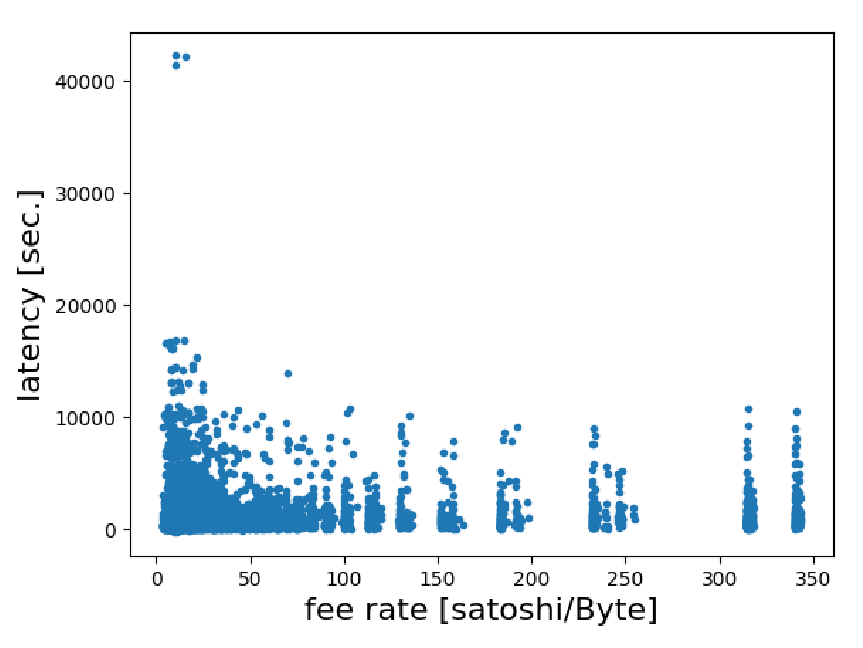
\includegraphics[width=85mm]{exp3-3.eps}
  \end{center}
  %\vspace{45mm}
  \caption{取引サイズに対する取引手数料の割合と取引がBCに取り込まれるまでにかかった時間の関係}
  \label{fig:exp3-3}
  %  \ecaption{english caption is here}
\end{figure}
%
割合(fee rate)が低いとBCに取引が取り込まれるまでに時間がかかっていることが分かる.
このことからSTNにおいても優先権付き待ち行列理論による考察は有効であると考えられる.



\section{Conclusion}
\label{sec:conclusion}

本研究ではBitcoin STNのノードを構築し,ブロックサイズの上限を撤廃した環境における取引処理に関するデータ分析や性能評価実験を行った.
取引処理の稼働率の時間変化を調べた結果,推定稼働率は殆どの時間帯において1を超えていることが分かった.
bitcoin-cliの機能を用いてBCの分岐確率の推定も行った結果,STNでは約8.5\%となり,BTCの4倍超の確率となっていることが分かった.
またP2Pネットワークの平均ブロック転送時間も約53秒と推定できた.
OP\_RETURNスクリプトを含む取引を1分に1回の高頻度で1週間の期間,転送することで取引処理性能を実験的に評価した.
その結果,取引がBCに取り込まれる確率は98\%であり,その時間分布は長期的には冪分布に従うような傾向が確認できた.
また優先権付き待ち行列の理論と矛盾しない3/2の冪指数に従う傾向も確認できた.
このことからSTNにおいても優先権付き待ち行列理論による考察は有効であると言える.

今後の課題としては,より大量な数の取引を長期間に渡って送信し続けた時の処理性能について確認することが挙げられる.



\begin{acknowledgement}
 This work was partially supported by the Japan Society for the Promotion of 
Science (JSPS) through KAKENHI (Grants-in-Aid for Scientific Research) Grant 
Number 20K11797. 
\end{acknowledgement}



%%
%\section*{Appendix}
%\addcontentsline{toc}{section}{Appendix}
%%
%%
%When placed at the end of a chapter or contribution (as opposed to at the end of the book), the numbering of tables, figures, and equations in the appendix section continues on from that in the main text. Hence please \textit{do not} use the \verb|appendix| command when writing an appendix at the end of your chapter or contribution. If there is only one the appendix is designated ``Appendix'', or ``Appendix 1'', or ``Appendix 2'', etc. if there is more than one.
%
%\begin{equation}
%a \times b = c
%\end{equation}


\begin{thebibliography}{99}

% Blockchain
\bibitem{HS1991}
  S. Haber and W. S. Stornetta, 
  ``How To Time-Stamp a Digital Document,''
  J. Cryptology, 3, 99-111 (1991)
  %\url{https://link.springer.com/content/pdf/10.1007\%2FBF00196791.pdf}

\bibitem{BHS1993}
  D. Bayer, S. Haber, and W. S. Stornetta,
  ``Improving the Efficiency and Reliability of Digital Time-Stamping,''
  Sequences II: Methods in Communication, Security, and Computer Sicence, 
  pp. 329-334 (1993).

\bibitem{HS1997}
  S. Haber and W. S. Stornetta, 
  ``Secure Names for Bit-Strings,''
  CCS'97: Proceedings of the 4th ACM conference on Computer and 
  communications security, pp. 28-35 (1997).
  %\url{https://nakamotoinstitute.org/static/docs/secure-names-bit-strings.pdf}


% Proof of Work
\bibitem{DN1993}
  C. Dwork and M. Naor, 
  ``Pricing via Processing or Combatting Junk Mail,''
  Advances in Cryptology (CRYPTO'92), 
  Lecture Notes in Computer Science, vol. 740, Springer (1993). 
  %\url{https://web.cs.dal.ca/~abrodsky/7301/readings/DwNa93.pdf}


\bibitem{JJ1999}
  M. Jakobsson and A. Juels, 
  ``Proofs of Work and Bread Pudding Protocols (Extended Abstract),''
  In: Preneel B. (eds) Secure Information Networks, 
  The International Federation for Information Processing, 
  vol 23, Springer (1999).
  %\url{https://www.arijuels.com/wp-content/uploads/2013/09/PoW.pdf}


% scalability problem
\bibitem{ZHZB2020}
  Q. Zhou, \textit{et al.}, 
  ``Solutions to Scalability of Blockchain: A Survey''
  IEEE Access, Vol. 8, pp.16440-16455, IEEE, 2020. 




% Bitcoin
\bibitem{nakamoto}
  S. Nakamoto, 
  ``Bitcoin: A Peer-to-Peer Electronic Cash System''
  (White paper), 2008 


\bibitem{btc}
  Bitcoin Core 
  \url{https://github.com/bitcoin/bitcoin}


\bibitem{Fujihara2018}
  A. Fujihara,
  ``Proposing a System for Collaborative Traffic Information Gathering and 
  Sharing Incentivized by Blockchain Technology,''
  The 10th International Conference on Intelligent Networking and 
  Collaborative Systems (INCoS-2018), pp.170-182 (2018)
  \url{https://link.springer.com/chapter/10.1007/978-3-319-98557-2_16}


\bibitem{Fujihara2019}
  A. Fujihara,
  ``PoWaP: Proof of Work at Proximity for a crowdsensing system for 
  collaborative traffic information gathering,'' 
  Internet of Things, 100046, Elsevier (2019).
  \url{https://www.sciencedirect.com/science/article/pii/S254266051830177X}

\bibitem{Fujihara2020}
  A. Fujihara, 
  ``Proposing a Blockchain-Based Open Data Platform and Its Decentralized Oracle,''
  Advances in Intelligent Networking and Collaborative Systems (INCoS2019), 
  Advances in Intelligent Systems and Computing, 
  Vol. 1035, pp. 190--201, Springer (2020).
  \url{https://link.springer.com/chapter/10.1007/978-3-030-29035-1_19}


\bibitem{YF2021a}
  T. Yanagihara and A. Fujihara, 
  ``Considering Cross-Referencing Method for Scalable Public Blockchain,''
  Advances in Internet, Data and Web Technologies, 
  Lecture Notes on Data Engineering and Communications Technologies, 
  Vol. 65, pp. 220-231, Springer (2021). 
  \url{https://link.springer.com/chapter/10.1007/978-3-030-70639-5_21}


\bibitem{YF2021b}
  T. Yanagihara and A. Fujihara,
  ``Cross-Referencing Method for Scalable Public Blockchain,''
  Internet of Things, Vol. 15, 100419 (2021). 
  \url{https://www.sciencedirect.com/science/article/pii/S2542660521000639}





\bibitem{PD2016}
  J. Poon and T. Dryja, 
  ``The Bitcoin Lightning Network: Scalable Off-Chain Instant Payments,'' 
  (2016) \url{https://lightning.network/lightning-network-paper.pdf}


\bibitem{silkroad}
  FBI, 
  ``Manhattan U.S. Attorney Announces Seizure of Additional \$28 Million 
    Worth of Bitcoins Belonging to Ross William Ulbricht, Alleged Owner 
    and Operator of ``Silk Road'' Website, '' 2013.
  \url{https://archives.fbi.gov/archives/newyork/press-releases/2013/manhattan-u.s.-attorney-announces-seizure-of-additional-28-million-worth-of}\\
  \url{-bitcoins-belonging-to-ross-william-ulbricht-alleged-owner-and}\\
  \url{-operator-of-silk-road-website}

\bibitem{alphabay}
  The US Department of Justice,
  ``AlphaBay, the Largest Online 'Dark Market,' Shut Down,'' 2017.
  \url{https://www.justice.gov/opa/pr/alphabay-largest-online-dark-market-shut-down}

\bibitem{welcome2video}
  The US Department of Justice,
  ``South Korean National and Hundreds of Others Charged Worldwide in the Takedown 
    of the Largest Darknet Child Pornography Website, Which was Funded by Bitcoin,'' 
  2019.
  \url{https://www.justice.gov/opa/pr/south-korean-national-and-hundreds-others-charged-worldwide}\\
  \url{-takedown-largest-darknet-child}



\bibitem{bloX}
  U. Klarman, \textit{et al.},
  ``bloXroute: A Scalable Trustless Blockchain Distribution Network''
  (White paper), 2018.
  \url{https://bloxroute.com/wp-content/uploads/2018/03/bloXroute-whitepaper.pdf}


\bibitem{bsv}
  Bitcoin SV (Satoshi Vision) 
  \url{https://github.com/bitcoin-sv/bitcoin-sv}

\bibitem{bitcoinscaling}
  Bitcoin Scaling Test Network
  \url{https://bitcoinscaling.io/}




\bibitem{OB2005}
  J. G. Oliveira and A.-L. Barab\'asi,
  ``Darwin and Einstein correspondence patterns,'' 
  Nature 437, 1251, 2005.


\bibitem{KK2019}
  S. Kasahara and J. Kawahara,
  ``Effect of Bitcoin fee on transaction-confirmation process,''
  Journal of Industrial and Management Optimization, 15 (1): 365-386, 2019.


\bibitem{woc}
  WhatsOnChain.com, BSV Explorer - STN,
  \url{https://stn.whatsonchain.com/}



% Flightradar24
\bibitem{flightradar24}
  Flight Tracker | Flightradar24 | Track Planes in Real-time,
  \url{https://www.flightradar24.com/}



\end{thebibliography}

\end{document}
